% !TeX root = ../main.tex

\section{Matlab}

\subsection{Basics}
    \begin{lstlisting}[language=Matlab, escapeinside=`', gobble=4]
    close all
    clear all
    clc

    addpath("../utils")

    % function definitions=========================================================
    f = @(x) (2 + exp(1)) * x .^ 2 + (2 * exp(1) + 1) * x - cosh(x - 1);

    % plot the function f==========================================================
    a = 0.5; b = 5.5;
    x_plot = linspace(a, b, 1000);
    figure, hold on, box on, grid on, axis equal;
    plot(x_plot, f(x_plot), "k-", "LineWidth", 1);
    xlabel("x","FontSize", 16)
    ylabel("f(x)","FontSize", 16)
    set(gca,"FontSize", 16)
    set(gca,"LineWidth", 1.5)

    % Errors behaviour=============================================================
    figure, semilogy(err1);

    % LU decomposition=============================================================
    [L, U, P] = lu(A);

    % Cholesky decompistion========================================================
    eigenvalues = eig(A);
    isreal(eigenvalues);
    all(eigenvalues > 0);
    R = chol(A);

    % Sparse matrix================================================================
    a = [1:10]';
    c = [10:19]';
    e = [102:111]';
    n = length(a);
    A_sparse = spdiags([e a c], [-1 0 1], n, n);
    % insert into diagonal (0), just below (-1) and just on top(1)
    % c on top will have first element (10) deleted
    % e below will have last element (111) deleted
    spy(A_sparse);

    % Condition number============================================================
    cond(A); % w.r.t. 2-norm or spectral norm
    cond(A,p); % w.r.t. p-norm
    cond(A,'inf'); % infinitu-norm
    condest(A_sparse); % 1-norm

    % Lagrange interpolation======================================================
    coeffs = polyfit(x,y,n) % x nodes, y targets, n degree of polynomial, but redundant
                            % for n data the degree is n-1, meaning least squares only
    d = polyval(coeffs,z) % evaluate interpolating polynomial at point z

    % Piecewise===================================================================
    d = interp1(x,y,z) % piecewise polynomial interpolation
    d = interp2(x,y,z) % cubic interpolation
    
    % Cubic spline================================================================
    d = spline(x,y,z) % cubic spline interpolation
    \end{lstlisting}

    Some util functions:
    \begin{lstlisting}[language=Matlab, escapeinside=`', gobble=4]
    function [x, x_iter] = bisection(f, a, b, tol)

    function [x, x_iter] = newton(f, df, x0, tol, Nmax)

    function [x, x_iter] = modified_newton(f, df, x0, tol, Nmax, m)

    function [xi, x_iter_bisection, x_iter_newton] = bisection_newton(f, df, a, b, tol_bisection, tol_newton, maxit_newton, multiplicity)

    function [xi, x_iter] = fixed_point(phi, x0, tol, maxit)

    function y = forward_substitution(L, b)

    function x = backward_substitution(U, b)

    function [L, U, x] = thomas(A_sparse, b)

    function [x, iter, incr] = stationary_method(B, g, x0, tol, max_it)

    function [x, iter, incr] = prec_rich_method(A, b, P, alpha, x0, tol, max_it)

    function int = midpoint(f, a, b)

    function int = composite_midpoint(f, a, b, m)

    function int = trapezoidal(f, a, b)

    function int = composite_trapezoidal(f, a, b, m)

    function int = simpson(f, a, b)

    function int = composite_simpson(f, a, b, m)
    \end{lstlisting}

\subsection{Nonlinear equations}
    \subsubsection{Manually retrieve roots intervals, bisection and error evaluation}
        Consider:
        $$
        \cot(x)=\frac{x^2-1}{2x}
        $$
        Define three intervals containing the three smallest positive roots
        
        \begin{lstlisting}[language=Matlab, escapeinside=`', gobble=8]]
        f = @(x) cot(x);
        g = @(x) (x .^ 2 - 1) ./ (2 * x);
        figure, hold on, box on, grid on;

        epsilon = 0.01;
        x_plot = linspace(0+epsilon, pi-epsilon, 1000);
        plot(x_plot, f(x_plot), "b-", "LineWidth", 1);
        x_plot = linspace(pi+epsilon, 2*pi-epsilon, 1000);
        plot(x_plot, f(x_plot), "b-", "LineWidth", 1);
        x_plot = linspace(2*pi+epsilon, 3*pi-epsilon, 1000);
        plot(x_plot, f(x_plot), "b-", "LineWidth", 1);

        x_plot = linspace(0+epsilon, 3*pi-epsilon, 1000);
        plot(x_plot, g(x_plot), "r-", "LineWidth", 2);

        % Three intervals for the roots are then [1,2], [3,4] and [6.5,7]
        % 6.5 as function discontinuous!
        \end{lstlisting}

        Apply bisection with tolerance of $10^{-6}$ then plot the evolution of the error function, remind that the error function is:
        $$
        |\alpha-x^{(k)}|
        $$
        \begin{lstlisting}[language=Matlab, escapeinside=`', gobble=8]
        tol = 1e-6;
        h = @(x) cot(x) - (x .^ 2 - 1) ./ (2 * x);
        [root1, x_iter1] = bisection(h, 1, 2, tol);

        % Since the exact value of the roots is NOT known, we perform
        % again the bisection method with a very small tolerance, and consider
        % the final approximation as the exact root of the equation.
        % First root
        [root1_precise, ~] = bisection(h, 1, 2, 1e-10*tol);
        err = abs(root1_precise - x_iter1);
        iter = numel(x_iter1);
        figure, box on, hold on, grid on;
        semilogy(err,"LineWidth",2);
        semilogy(tol*ones(iter,1), "r--","LineWidth",2);
        xlim([0 iter+1])
        set(gca,"FontSize",16)
        xlabel("Iteration","FontSize",16)
        ylabel("Error","FontSize",16)
        \end{lstlisting}

    \subsubsection{Fixed point method}
        Solve $x^2-5=0$ to find the root $\alpha=\sqrt{5}$ using the following iterative methods:
        \begin{enumerate}
            \item $x^{(k+1)}=5+x{(k)}-\left(x^{(k)}\right)^2$
            \item $x^{(k+1)}=1+x^{(k)}-\frac{1}{5}\left(x^{(k)}\right)^2$
        \end{enumerate}
        \begin{lstlisting}[language=Matlab, escapeinside=`', gobble=8]
        % fixed point convergent if |phi'(alpha)| < 1, if > 1 diverges, if == 1 idk
        a = sqrt(5);
        f = @(x) x .^ 2 - 5;

        phi1 = @(x) 5 + x - x .^ 2;
        % check consistency, phi(alpha) == alpha
        phi1(alpha) == alpha
        dphi1 = @(x) 1 - 2 * x;
        abs(dphi1(a))

        phi2  = @(x) 1 + x - 1/5*x.^2;
        dphi2 = @(x) 1 - 2/5*x;
        abs(dphi2(a))

        % phi2 converges:
        tol = 1e-6;
        maxit = 1000;
        x0 = a + 2*rand(0.001); % random initial value in [a,a+0.001]
        x0 = a + 0.001; % intial guess
        [x, x_iter] = fixed_point(phi2, x0, tol, maxit);
        \end{lstlisting}

    \subsubsection{Fixed point method: scheme consistency}
        Given the equation:
        $$
        f(x)=e^{x^2}\log(x+1)=1
        $$
        The equation is defined for $x>-1$. Consider:
        $$
        x^{(k+1)}=\sqrt{-\log\log\left(x^{(k)}+1\right)}
        $$
        Compute the root with tolerance of $10^{-3}$.

        The method is defined only if:
        $$
        -\log\log\left(x^{(k)}+1\right) \geq 0
        $$
        $$
        \log\log\left(x^{(k)}+1\right) \leq 0
        $$
        $$
        0<\log\left(x^{(k)}+1\right) \leq 1
        $$
        $$
        1<\left(x^{(k)}+1\right) \leq e
        $$
        $$
        0<x^{(k)} \leq e-1
        $$
        It's derivative is:
        $$
        \frac{1}{2}\cdot
        \sqrt{-\log\log\left(x^{(k)}+1\right)}
        \cdot
        \left(
            -\frac{
                \frac{
                    1
                }{
                    x^{(k)}+1
                }
            }{\log\left(x^{(k)}+1\right)}
        \right)
        $$
        $$
        \frac{1}{
            2
            \left(x^{(k)}+1\right)
            \log\left(x^{(k)}+1\right)
            \sqrt{-\log\log\left(x^{(k)}+1\right)}
        }
        $$
        \begin{lstlisting}[language=Matlab, escapeinside=`', gobble=8]
        x_plot = linspace(-1+0.001,2,1000);

        f = @(x) exp(x.^2).*log(x + 1) - 1;

        % find the interval containing the root
        figure, hold on, grid on, box on; %axis equal;
        plot(x_plot,f(x_plot),"r-");
        plot(x_plot,zeros(size(x_plot)),"b-");

        % interval in [0.5 1]
        x_plot = linspace(0.5, 1, 1000);

        bisector = @(x) x;
        % to check if method consistent look at the bisector/slope of derivative
        % In this case in a neighborhood of the root, the absolute
        % value of the derivative is less than 1
        % ATTRACTOR
        phi1 = @(x) sqrt(-log(log(x + 1)));
        figure, hold on, grid on, box on, axis equal;
        plot(x_plot,phi1(x_plot),"r-");
        plot(x_plot, bisector(x_plot),"b-");

        % alternatively plot the derivative
        dphi1 = @(x) -1./(2*log(x + 1).*(-log(log(x + 1))).^(1/2).*(x + 1));
        figure, hold on, grid on, box on, axis equal;
        plot(x_plot,abs(dphi1(x_plot)),"r-");
        plot(x_plot,ones(size(x_plot)),"b-");

        % So here we can apply fixed point
        [xi1, x1] = fixed_point(phi1, 0.9, 1e-3, 1000);
        xi1
        iter1 = numel(x1)
        \end{lstlisting}
        \begin{center}
            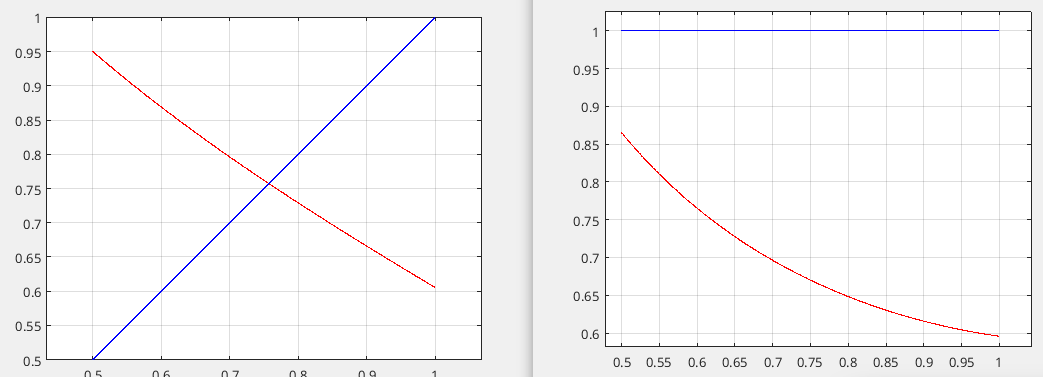
\includegraphics[width=1\textwidth]{images/code_fixed_bisector.png}            
        \end{center}

        Consider this other method:
        $$
        x^{(k+1)}=x^{(k)}e^{\left(x^{(k)}\right)^2}\log(x^{(k)}+1)
        $$
        \begin{lstlisting}[language=Matlab, escapeinside=`', gobble=8]
        % The comparison with the slope of the bisector shows that,
        % in a neighborhood of the root, the absolute
        % value of the derivative is greater than 1
        % For this reason the method will not converge.
        % REPULSOR
        phi2 = @(x) x .* exp(x .^ 2) .* log(x + 1);
        figure, hold on, grid on, box on, axis equal;
        plot(x_plot, phi2(x_plot), "r-");
        plot(x_plot, bisector(x_plot), "b-")
        \end{lstlisting}
        \begin{center}
            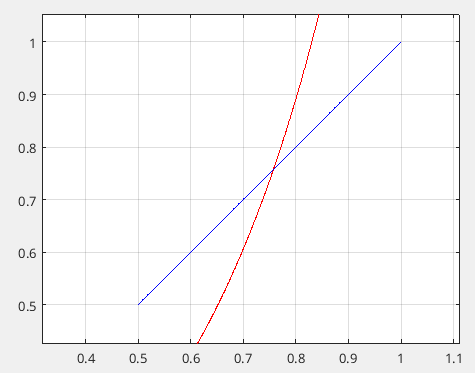
\includegraphics[width=0.6\textwidth]{images/code_fixed_bisector2.png}            
        \end{center}

        Now consider Newton method, verify the consistency of the scheme and compute the convergence orders, remid that:
        $$
        p=\frac{
            \log\left[
                \frac{e^{k+2}}{e^{k+1}}
            \right]
        }{
            \log\left[
                \frac{e^{k+1}}{e^k}
            \right]
        }
        $$
        \begin{lstlisting}[language=Matlab, escapeinside=`', gobble=8]
        phi1 = @(x) sqrt(-log(log(x + 1)));
        [xi1, x_iter_fixed] = fixed_point(phi1, 0.9, 1e-3, 1000);
        
        % The plot of f shows that f'(x) is always positive in [-1, 2], therefore the method is locally convergent.
        df = @(x) 2.*x.*exp(x.^2).*log(x+1) + exp(x.^2)./(x+1);
        [x_newton, x_iter_newton] = newton(f, df, 1.4, 1e-3, 1000);
        
        % Rate of convergence
        [xiex, xex] = newton(f, df, 1.4, 1e-12, 1000);
        err1 = abs(x_iter_fixed - xiex);
        err3 = abs(x_iter_newton - xiex);
        
        % Approximate the convergence order
        p1 = diff( log(err1(2:end) ) ) ./ diff( log(err1(1:end-1) ) )
        p3 = diff( log(err3(2:end) ) ) ./ diff( log(err3(1:end-1) ) ) 
        
        % Or compute normally
        p1 = log(err1(end)/err1(end-1))./log(err1(end-1)/err1(end-2))
        p3 = log(err3(end)/err3(end-1))./log(err3(end-1)/err3(end-2))
        
        % The order of the first method is 1, Newton method is as expected of second order.
        figure, hold on, box on;
        semilogy(err1, 'bs-',"LineWidth",2)
        semilogy(err3, 'rs-',"LineWidth",2)
        set(gca,"LineWidth",1.5)
        set(gca,"FontSize",16)
        xlim([0 numel(err1)+1])
        xlabel("iterations","FontSize",16)
        ylabel("error","FontSize",16)
        h = legend('Method 1','Newton');
        set(h,"FontSize",16)
        \end{lstlisting}
        \begin{center}
            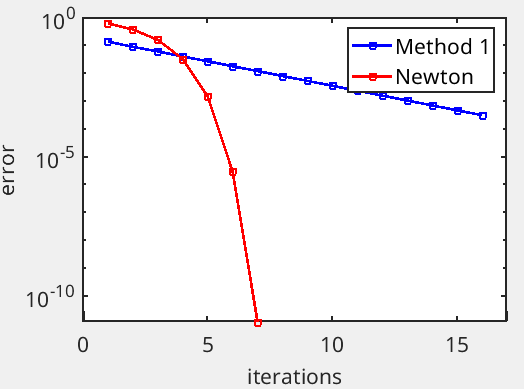
\includegraphics[width=0.6\textwidth]{images/code_fixed_bisector3.png}            
        \end{center}

\subsection{Systems of Linear Equations: Direct Methods}
    \subsubsection{Solve with LU}
        Solve the system $Ax=b$ and compute the determinant of $A$
        \begin{lstlisting}[language=Matlab, escapeinside=`', gobble=8]
        A = [2 10 4 0;
            1  0 2 2;
            1 4 0 2;
            1 2 1 1];
        b = [10 1 3 3]';
       
        [L, U] = lu(A);
        % In this case it is not essential to include the matrix P among the output
        % variables in order to have L in the form of a lower triangular matrix
        % with L_ii = 1 for each i.
        
        y = L \ b; %forward
        x = U \ y; %backward
       
        % or use
        y = forward_substitution(L, b)
        x = backward_substitution(U, b)
        
        % Check
        A \ b
        
        % Thanks to the Binet-Cauchy formula, we have, for generic square matrices,
        % det(A*B) = det(A)*det(B).
        % In our case, since A = L*U, det(A) = det(L*U) = det(L)*det(U).
        % However L_ii = 1 for each i, so det(L) = 1
        % => det(A) = det(U).
        
        detA = prod(diag(U))
        
        % Check with the command det
        det(A)
        \end{lstlisting}

        Solve now the system with a new $b$
        \begin{lstlisting}[language=Matlab, escapeinside=`', gobble=8]
        b_new = [-22 -12 -1 -11]';    

        % we don't need to recompute the LU factorization
        y2 = forward_substitution(L, c);
        x2 = backward_substitution(U, y2);
        \end{lstlisting}
    
    \subsubsection{Custom inverse}
        Write a function that computes the inverse of a generic square matrix
        \begin{lstlisting}[language=Matlab, escapeinside=`', gobble=8]
        function [InvA] = MyInv(A)
            [L,U] = lu(A);
            %s = size(A);
            %n = s(1);
            n = length(A);
            for k = 1:n
                e = zeros(n,1);
                e(k) = 1;
                y = forward_substitution(L,e);
                InvA(:,k) = backward_substitution(U,y); 
            end
        end
        \end{lstlisting}

    \subsubsection{LU conditions and pivoting}
        Consider matrix $E$ with $b$:
        $$
        E=\begin{bmatrix}
            4 & 1 & 1 & 1 & 5\\
            4 & 1 & 2 & 0 & 0\\
            1 & 0 & 15 & 5 & 1\\
            0 & 2 & 4 & 10 & 2\\
            3 & 1 & 2 & 4 & 20
        \end{bmatrix}
        \qquad
        A=\begin{bmatrix}
            12\\
            19\\
            22\\
            18\\
            30
        \end{bmatrix}
        $$
        Verify that the sufficient conditions for the existence and uniqueness of the LU decomposition without pivoting are NOT fulfilled by $E$
        \begin{lstlisting}[language=Matlab, escapeinside=`', gobble=8]
        E = [4 1 1 1 5;
            4 1 2 0 0;
            1 0 15 5 1;
            0 2 4 10 2;
            3 1 2 4 20];

        b = [12 19 22 18 30]';

        n = length(E(1,:));

        % Let calculate the determinant of the all the minor fo the matrix E

        for i = 1:n-1
            det(E(1:i, 1:i))
        end

        % Since one of the minor determinants is equal to zero, the LU
        % factorization without pivoting does not exist!

        % ATTENTION
        % if a matrix E does not admit a LU factorization and you
        % call lu command without the output P, matlab does not 
        % return the lu factorization of P*E but a factorization
        % of E which is not lower-upper triangular
        [L, U] = lu(E);
        detA = prod(diag(U))
        L % is not triangular!
        spy(L)
        \end{lstlisting}

        Compute the LU and verify if pivoting takes place, then solve the system
        \begin{lstlisting}[language=Matlab, escapeinside=`', gobble=8]            
        [L, U, P] = lu(E);
        detA = prod(diag(U))
        spy(L)
        P % is not the identity matrix => pivoting is needed

        y = forward_substitution(L,P*b); %L\(P*b); 
        x = backward_substitution(U,y); %U\y

        x2 = E \ b

        x == x2 % precision errors, but should be correct
        \end{lstlisting}
        
    \subsubsection{Cholesky decomposition}
        Verify that the Cholesky decomposition can be applied to matrix $A$ (is spd), then solve the system

        \begin{lstlisting}[language=Matlab, escapeinside=`', gobble=8]
        A = [44 15 29 26 119;
            15 33 32 18 15;
            29 32 252 112 73;
            26 18 112 124 90;
            119 15 73 90 430];
        b = [1 1 1 1 1]';
       
        % A must be spd:
        % - all eigenvalues are real (s)
        % - all eigenvalues are > 0 (pd)
        eigenvalues = eig(A);
        isreal(eigenvalues);
        all(eigenvalues > 0);
        
        R = chol(A);
        
        y = forward_substitution(R',b); % R'\b
        x = backward_substitution(R,y); % R\y
        \end{lstlisting}
    
    \subsubsection{Sparse matrix and Thomas algorithm}
        Consider the tridiagonal matrix $A\in\mathbb{R}^{10\times 10}$
        $$
        A=\begin{bmatrix}
            1 & 11\\
            102 & 2 & 12\\
            & 103 & 3 & 13\\
            & \cdots & \cdots & \cdots\\
            &  & 109 & 9 & 19\\
            &  &  & 110 & 10
        \end{bmatrix}
        $$
        Then consider the linear system $Ax=b$ such that $x=[1\cdots 1]\in\mathbb{R}^{10\times 1}$. Store the matrix in a sparse format and check the solution of the linear system with Thomas
        \begin{lstlisting}[language=Matlab, escapeinside=`', gobble=8]
        a = [1:10]';
        c = [10:19]';
        e = [102:111]';
        n = length(a);
        A_sparse = spdiags([e a c], [-1 0 1], n, n)
        % insert into diagonal (0), just below (-1) and just on top(1)
        % c on top will have first element (10) deleted
        % e below will have last element (111) deleted

        % alternative way to create A as a sparse and full matrix
        % A = diag(1:10) + diag(102:110,-1) + diag(11:19, 1)
        % Asparse = sparse(A)
        x = ones(n,1);
        b = A_sparse*x

        [L, U, x_test] = thomas(A_sparse, b);
        A_sparse \ b
        x_test
        \end{lstlisting}

    \subsubsection{Condition number}
        Consider the linear system $Ax=b$:
        $$
        A=\begin{bmatrix}
            1 & 0 & 0\\
            0 & 1 & 0\\
            0 & 0 & \epsilon
        \end{bmatrix}
        \qquad
        b=\begin{bmatrix}
            1\\
            0\\
            0
        \end{bmatrix}
        $$
        Compute the condition number for $p=1,2,\infty$, the perturbation on the solution with $\delta b=\begin{bmatrix}
            0 & 0 & \alpha
        \end{bmatrix}^T$ and verify the perturbation relation with the infinity norm
        $$
        \frac{||\delta x||}{||x||}\leq
        \underlabel{
            \sqrt{\frac{
                \lambda_{max}(A^TA)
            }{\lambda_{min}(A^TA)}}
        }{$K(A)\geq 1$ condition number}    
        \frac{||\delta b|}{||b||}
        $$
        $$
        \epsilon=10^{-6}
        \qquad
        \alpha=10^{-12},\,\,10^{-6}
        $$
        \begin{lstlisting}[language=Matlab, escapeinside=`', gobble=8]
        epsilon = rand() / 1000;
        epsilon = 1e-6;
        
        for alpha = [1e-6 1e-12]
            A = eye(3);
            A(3, 3) = epsilon;
        
            b = [1 0 0]';
        
            % exact solution
            x = A \ b;
        
            % condition number
            % Since A is symmetric, norm-1 == norm-inf
            K_1 = cond(A, 1)
            cond(A, 2);
            cond(A);
            K_inf = cond(A, 'inf')
        
            % associated solution with perturbation on b
            delta_b = [0 0 alpha]';
            delta_x = A \ delta_b;
        
            % verify inequality on condition number:
            norm(delta_x,inf) / norm(x,inf) <= K_inf * norm(delta_b,inf) / norm(b,inf)
        end
        \end{lstlisting}

    \subsubsection{Condition number by trials}
        Consider the Hilbert matrix of order $n=10,20,40$, estimate $K_2(H_n)$ using the technique of perturbating a linear system. 
        \begin{lstlisting}[language=Matlab, escapeinside=`', gobble=8]
        for n = [10,20,40]
            H = hilb(n)
            x = ones(n, 1);
            b = H * x;
            % condition number by trials
            pert_mag = 1e-6; % Perturbation magnitude
            n_trials = 100;
            KH_est = 0;
        
            for ii = 1:n_trials
                deltab = randn(n, 1) * pert_mag;
                deltax = H \ deltab;
                KH_est_ii = norm(deltax) / norm(x) * norm(b) / norm(deltab);
                KH_est = max(KH_est_ii, KH_est);
            end
            K_2 = cond(H)
        end
        % The estimates obtained are lower. This is expected, since
        % the condition number represents the maximum 
        % possible amplification of the relative error on data. With the first
        % approach we might not have considered the worst condition, 
        % hence the estimate is lower than the result with cond command.

        KH(ii) = cond(H);
        err(ii) = norm(x - x_ex) / norm(x);
        \end{lstlisting}
    
\subsection{Systems of Linear Equations: Iterative Methods}
    \subsubsection{Stationary Richardson schemes: Jacobi and Gauss-Seidel}
        Reminder, we want
        $$
        x^{(k+1)}=
        \underlabel{\alpha_kP^{-1}b}{$g_{\alpha_k}$}+
        \underlabel{\left(
            I-\alpha_kP^{-1}A
            \right)}{$B_{\alpha_k}$}x^{(k)}
        $$
        $$
        A = D-E+(A-(D-E))
        $$
        With $E$ lower triangular part, $D$ diagonal of $A$ and $\alpha=1$
        $$
        \text{Jacobi}
        \qquad
        \qquad
        \qquad
        \qquad
        \qquad
        \text{Gauss-Seidel}
        $$
        $$
        x^{(k+1)}=\underlabel{(I-D^{-1}A)}{
            $B_J$
        }x^{(k)}+\underlabel{D^{-1}b}{
            $g_J$
        }
        \qquad
        x^{(k+1)}=\underlabel{(I-(D-E)^{-1}A)}{$B_{GS}$}x^{(k)}+
        \underlabel{(D-E)^{-1}b}{$g_{GS}$}
        $$
        Study the convergece for Jacobi, then apply stationary method to check the result with $x_0=[0,0,0]^T$, tol=$10^{-6}$ and maxit=100
        \begin{lstlisting}[language=Matlab, escapeinside=`', gobble=8]
        A = [
            2 1 -2;
            1 2 1;
            2 1 2
            ];
        x = [1 2 3]';
        b = inv(A) \ x;

        % JACOBI
        % A = D-E+(A-(D-E))
        % where D=diagonal part of A=diag(A)
        % where E lower triagular part
        % B = inv(D)*(D-A)
        % g = inv(D)*b
        % BUT WE CANNOT USE inv(), but as D is diagonal, inv(D) = 1/D

        D = diag(diag(A));
        B_j = D \ (D - A);
        g_j = D \ b;

        % matrix are not particular (not spd), to check convergence
        % compute the 2norm of iteration matrices
        normB_j = norm(B_j);

        % If bigger than 1, compute spectral radius
        rhoB_j = max(abs(eig(B_j)))

        % If a spectral norm > 1, the method will not converge
        % Finally solve the system
        x0 = [0 0 0]';
        tol = 1.e-6;
        max_it = 100;
        [x, iter, incr] = stationary_method(B_j, g_j, x0, tol, max_it);

        x1j = B_j*x0 + g_j;
        k_j_min = log(tol*(1 - normB_j)/norm(x-x0)) / log(norm_Bj);
        \end{lstlisting}

        Study the convergece for Gauss-Seidel, then apply stationary method to check the result with $x_0=[0,0,0]^T$, tol=$10^{-6}$ and maxit=100
        \begin{lstlisting}[language=Matlab, escapeinside=`', gobble=8]
        % GAUSS-SEIDEL
        % g = inv(D-E)*b
        % How to find inv(D-E) without inv()?
        % If we have inv(A)w=z, we can both multiply by A
        % A*inv(A)w = A*z -> w=Az, so z = A\b!!!
        % So for use g = (D-E)\b
        % Same holds for matrices, inv(A)*B = C -> C = A\B
        
        E = -tril(A, -1);
        % -1 will put diagonal at 0 and uppertriangular 0
        % L = tril(A, -1);
        % U = triu(A, 1);
        
        B_gs = (D - E) \ (D - E - A);
        g_gs = (D - E) \ b;
        
        % matrix are not particular (not spd), to check convergence
        % compute the 2norm of iteration matrices
        
        normB_gs = norm(B_gs);
        
        % If bigger than 1, compute spectral radius
        rhoB_gs = max(abs(eig(B_gs)));
        
        % If a spectral norm > 1, the method will not converge
        % Finally solve the system
        x0 = [0 0 0]';
        tol = 1.e-6;
        max_it = 100;
        [x, iter, incr] = stationary_method(B_gs, g_gs, x0, tol, max_it);

        x1gs = B_gs*x0 + g_gs;
        k_gs_min= log(tol*(1 - normB_gs)/norm(x1gs-x0)) / log(normB_gs);
        \end{lstlisting}

    \subsubsection{Jacobi iterations}
        Using Jacobi, compute how many iterations are required to ensure that the infinity norm of the error is less than $10^{-9}$
        \begin{lstlisting}[language=Matlab, escapeinside=`', gobble=8]
        n = 3;
        alpha = 1e-4;
        A = eye(n);
        A(1, n) = 1 / alpha;
        
        D = diag(diag(A));
        
        B = D \ (D - A);        
        b = ones(n, 1);
        g = D \ b;
        
        % check if Jacobi will converge or not
        norm(B)
        max(abs(eig(B)))
        
        % infinity norm on the error ~ check increment
        iter = 0;
        x = b;
        dx = b;        
        while norm(dx, inf) >= 1e-9
            x_old = x;
            x = B * x + g;
            dx = x - x_old;
            iter = iter + 1;
        end
        
        iter
        \end{lstlisting}
    
    \subsubsection{Choice of $\alpha$ of the Richardson method}
        Remind that:
        $$
        B=(I-\alpha P^{-1}A)
        \qquad
        \alpha_{opt}=\frac{
            2
        }{
            \lambda_{\max}(P^{-1}A)+\lambda_{\min}(P^{-1}A)
        }
        $$
        Check if matrices $A$ and $T$ are spd, then apply Richardson first with $\alpha=0.2,0.33$ with $P=I$ then with $\alpha_{opt}$ with $P=T$
        \begin{lstlisting}[language=Matlab, escapeinside=`', gobble=8]
        n = 50;
        diagonal = 4 * ones(n, 1);
        minus = -ones(n, 1);
        A = spdiags([minus minus diagonal minus minus], [-2 -1 0 1 2], n, n);
        A = full(A);
        T = spdiags([minus minus * -2 minus], [-1 0 1], n, n);
        T = full(T);
        b = 0.2 * ones(n, 1);
        
        % spd? yes
        isreal(eig(A))
        all(eig(A) > 0)
        
        isreal(eig(T))
        all(eig(T) > 0)
        
        % converge, check if spectral radius of B < 1
        % with P = I -> B = I-alpha*I^-1*A
        tol = 1e-6;
        x0 = zeros(n, 1);
        P = eye(n);
        maxit = 10000;
        
        for alpha = [0.2 0.33]
            B = eye(n) - alpha * (P \ A);
            if max(abs(eig(B))) < 1
                disp(["Converges for ", alpha])
                [x, iter, incr] = prec_rich_method(A, b, P, alpha, x0, tol, maxit);
                x
                iter
            end
        end
        
        % alpha_opt
        P = T;
        eig_max = max(eig(P \ A));
        eig_min = min(eig(P \ A));
        alpha_opt = 2 / (eig_max + eig_min);
        B = eye(n) - alpha_opt * (P \ A);
        max(abs(eig(B)))
        [x, iter, incr] = prec_rich_method(A, b, P, alpha_opt, x0, tol, maxit);
        x
        iter
        \end{lstlisting}
    
\subsection{Approximation of Functions and Data}
    \subsubsection{Equally spaced nodes: Lagrange, piecewise and cubic spline}
        Approximate the function $f(x)=x\sin(x)$ in the interval $[-2,6]$. Consider a set of equally spaced nodes: find the interpolating polynomial using Lagrange basis polynomials of degree 4, 6, 8. Then estimate the interpolation error when resorting to quadratic interpolation ($n=2$). Evaluate the interpolating polynomial in 1000 equally spaced points. Remind that the interpolating error:
        $$
        h=\frac{x_n-x_0}{n}
        $$
        $$
        \max_{x\in I}\left|E_nf(x)\right|
        \leq
        \underlabel{
            \frac{
                h^{n+1}
            }{
                4(n+1)
            }
        }{A}
        \cdot
        \underlabel{
            \max_{x\in I}\left|
                f^{(n+1)}(x)
            \right|
        }{B}
        $$
        \begin{lstlisting}[language=Matlab, escapeinside=`', gobble=8]
        f = @(x) x .* sin(x);
        x_plot = linspace(-2, 6, 1000);
        
        figure, hold on, box on, grid on, axis equal;
        plot(x_plot, f(x_plot), 'k--', 'Linewidth', 2);
        
        for n = [4 6 8]
            num_nodes = n + 1;
            x_nodes = linspace(-2, 6, num_nodes);
            y_nodes = f(x_nodes);
            coeff = polyfit(x_nodes, y_nodes, n);
            interp_plot = polyval(coeff, x_plot);
            if n == 4
                plot(x_plot, interp_plot, 'r-');
            end
            if n == 6
                plot(x_plot, interp_plot, 'b-');
            end
            if n == 8
                plot(x_plot, interp_plot, 'g-');
            end
        end
        
        h = legend("Original", "Degree 4", "Degree 6", "Degree 8");
        set(h, "FontSize", 12);
        
        % interpolation error when resorting to a quadratic interpolation, n=2
        % which means n+1=3 num_nodes
        n = 2;
        x_nodes = linspace(-2, 6, n + 1);
        y_nodes = f(x_nodes);
        coeff = polyfit(x_nodes, y_nodes, n);
        interp_plot = polyval(coeff, x_plot);
        figure, hold on, box on, grid on, axis equal, xlim auto, ylim auto;
        
        plot(x_plot, f(x_plot), 'k--', 'Linewidth', 1);
        plot(x_plot, interp_plot, 'r');
        
        h = 6 - (-2) / n;
        
        % compute third derivative
        f_1 = @(x) sin(x) + x .* cos(x);
        f_2 = @(x) 2 * cos(x) - x .* sin(x);
        f_3 = @(x) -2 * sin(x) - sin(x) + x .* cos(x);
        
        err = (h ^ (n + 1) / 4 * (n + 1)) * max(f_3(x_plot));
        plot(x_plot, abs(f(x_plot) - interp_plot), 'Linewidth', 2);
        h = legend("Original", "Quadratic", "Error");
        set(h, "FontSize", 12);
        \end{lstlisting}
        \begin{center}
            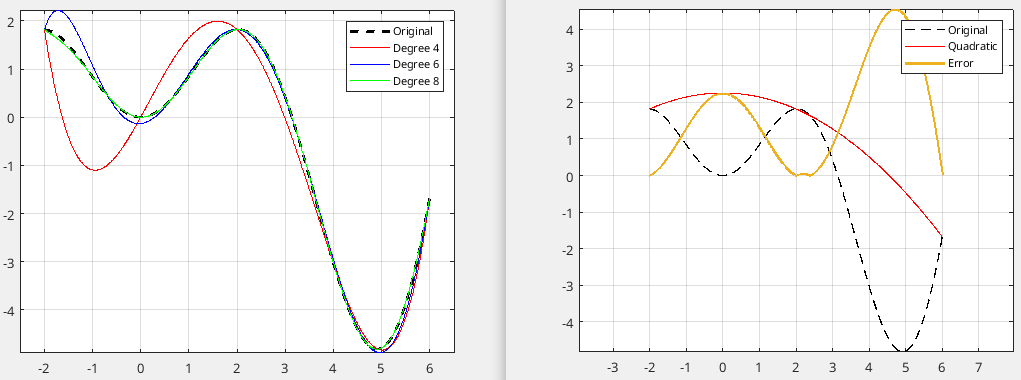
\includegraphics[width=1\textwidth]{images/code_interp_lagrange.png}            
        \end{center}
        Now compute the piecewise linear interpolant and the cubic spline with $n+1=6,11,21$ equally spaced nodes
        \begin{lstlisting}[language=Matlab, escapeinside=`', gobble=8]
        % Piecewise linear interpolant and cubic spline with n+1=6,9,21 equally space nodes
        for n = [5 8 20]
            figure, hold on, box on, grid on, axis equal, xlim auto, ylim auto;
            plot(x_plot, f(x_plot), 'k--', 'Linewidth', 1);
        
            num_nodes = n + 1;
            x_nodes = linspace(-2, 6, num_nodes);
            y_nodes = f(x_nodes);
        
            % (x_nodes, y_nodes) pairs, directly evaluate on x_plot
            piecewise_plot = interp1(x_nodes, y_nodes, x_plot);
            spline_plot = spline(x_nodes, y_nodes, x_plot);
        
            plot(x_plot, piecewise_plot, 'r-');
            plot(x_plot, spline_plot, 'b-');
            legend_1 = strcat("Piecewise ", num2str(n), " nodes");
            legend_2 = strcat("Cubic spline ", num2str(n), " nodes");
            h = legend("Original", legend_1, legend_2);
            set(h, "FontSize", 8);
        end
        \end{lstlisting}
        \begin{center}
            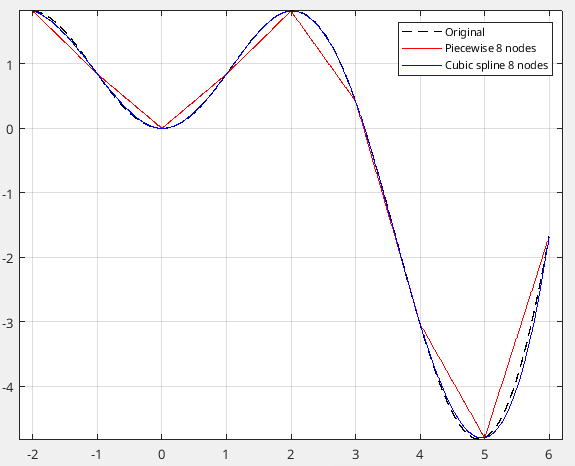
\includegraphics[width=0.6\textwidth]{images/code_interp_piece_spline.png}
        \end{center}
    
    \subsubsection{Runge, Chebyshev nodes and convergence order}
        Consider the function:
        $$
        f(x)=\frac{1}{1+x^2}
        \qquad
        -5\leq x \leq 5
        $$
        Verify the Runge phenomenon
        \begin{lstlisting}[language=Matlab, escapeinside=`', gobble=8]
        a = -5;
        b = 5;
        f = @(x) 1 ./ (1 + x .^ 2);
        x_plot = linspace(a, b, 1000);
        figure, hold on, grid on, axis equal, box on;
        plot(x_plot, f(x_plot), 'k--');
        
        % plot with n=2:2:10
        for n = 2:2:10
            x_nodes = linspace(a, b, n + 1);
            y_nodes = f(x_nodes);
            coeff = polyfit(x_nodes, y_nodes, n);
            interp_plot = polyval(coeff, x_plot);
            plot(x_plot, interp_plot, '"r-");
        
            % Runge phenomenon, the max of n-derivative of f
            % goes to +inf quicker than A goes to 0
            n
            norm(f(x_plot) - interp_plot, inf)
        end
        \end{lstlisting}

        Compute the piecewise linear interpolation with $n=1,2,4,8,16,32$ subintervals and plot the result. Find the error w.r.t. the infinity norm and verify that it converges quadratically as a function of the distance between two nodes
        \begin{lstlisting}[language=Matlab, escapeinside=`', gobble=8]
        % piecewise linear
        exp = 0:5;
        n_vect = (2 * ones(1, exp(end) + 1)) .^ exp;

        for i = 1:numel(n_vect)
            n = n_vect(i);
            x_nodes = linspace(a, b, n + 1);
            y_nodes = f(x_nodes);
            piece_plot = interp1(x_nodes, y_nodes, x_plot);

            % figure, hold on, grid on, axis equal, box on;
            % plot(x_plot, f(x_plot), "k--");
            % plot(x_plot, piece_plot, "r-");
            error(i) = norm(f(x_plot) - piece_plot, inf);
        end

        % determination of the element width
        H = (b - a) ./ n_vect;
        figure, hold on, grid on, axis equal, box on;
        loglog(H, error, "bx-", "LineWidth", 2, "MarkerSize", 8);
        loglog(H, H, "r-", "LineWidth", 2);
        loglog(H, H .^ (2), "g-", "LineWidth", 2);
        xlabel("h", "FontSize", 16)
        ylabel("error", "FontSize", 16)
        legend("error", "O(h)", "O(h^2)");
        xlim([min(H), 1]);
        ylim([min(error), 1]);
        % THIS LEGEND REQUIRED
        % to understand behavior at infinite we have to increase the number of subinterval
        % increase n_vect [1 2 4 8 16 32 64 128];
        % look at the line that at the BEGINNING is ALMOST parallel to the error line

        % compute convergence order with:
        order = (log(error(1:end - 1) ./ error(2:end)) / log(2))'
        % or using the diff command build in in matlab
        p = -diff(log(error)) / log(2)
        \end{lstlisting}
        \begin{center}
            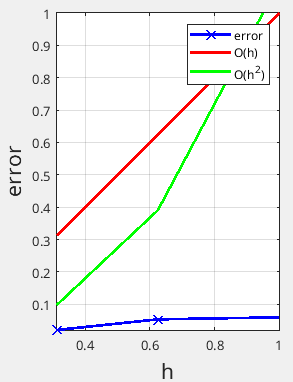
\includegraphics[width=0.4\textwidth]{images/code_runge_error.png}
        \end{center}

        Compute how many equally spaced nodes are needed in order to ensure an interpolation error with infinity norm smaller than $10^{-3}$. Remind that for piecewise:
        $$
        \max_{x\in I}\left|E_1^Hf(x)\right|
        \leq
        \frac{
            H^2
        }{
            8
        }\cdot
        \max_{x\in I}\left|
            f''(x)
        \right|\qquad
        f\in C^2(\overline{I})
        $$
        \begin{lstlisting}[language=Matlab, escapeinside=`', gobble=8]
        % or use the formula
        df1 = ...;
        df2 = ...;
        max_val = max(df2(x_plot));
        H = sqrt(8 * 1e-3 / max_val);
        n = ceil((b - a) / H); % degree
        n + 1
        \end{lstlisting}

        Compute $\Pi_nf(x)$ using Chebyshev nodes:
        $$
        x_i=\frac{a+b}{2}+\frac{b-a}{2}\hat{x}_i
        \qquad
        \hat{x}_i=-\cos(\pi i/n),\,\,i=0,\cdots,n
        $$
        \begin{lstlisting}[language=Matlab, escapeinside=`', gobble=8]
        % Chebyshev nodes
        exp = 0:5;
        n_vect = (2 * ones(1, exp(end) + 1)) .^ exp;
        
        for i = 1:numel(n_vect)
            n = n_vect(i);
        
            % Calculation of the Chebyshev nodes
            indexes = 0:n;
            x_hat = -cos(pi * indexes / n);
            x_nodes = (a + b) / 2 + (b - a) / 2 .* x_hat;
            y_nodes = f(x_nodes);
        
            coeff = polyfit(x_nodes, y_nodes, n);
            chebyshev_plot = polyval(coeff, x_plot);
            % figure, hold on, grid on, axis equal, box on;
            % plot(x_plot, f(x_plot), "k--");
            % plot(x_plot, chebyshev_plot, "r-");
            error(i) = norm(f(x_plot) - chebyshev_plot, inf);
        end
        
        H = (b - a) ./ n_vect;
        % A second order convergence cannot be expected, since the function is not smooth enough.
        % Calculation of the error
        order = (log(error(1:end - 1) ./ error(2:end)) / log(2))'
        % or using the diff command build in in matlab
        p = -diff(log(error)) / log(2)            
        \end{lstlisting}
        
    \subsubsection{Least squared approximation}
        Remind that degree $m<<n$, if $m==n$ we have Lagrange.
        \begin{lstlisting}[language=Matlab, escapeinside=`', gobble=8]
        a = -1;
        b = 1;
        f = @(x) abs(x - pi / 12);
        x_plot = linspace(a, b, 1000);
        figure, hold on, grid on, axis equal, box on;
        plot(x_plot, f(x_plot), 'k--');

        % runge
        for n = 2:2:10
            x_nodes = linspace(a, b, n + 1);
            y_nodes = f(x_nodes);
            coeff = polyfit(x_nodes, y_nodes, n);
            poly_plot = polyval(coeff, x_plot);
            plot(x_plot, poly_plot, "r-");
        end

        % use least squares approach with number of nodes = 10
        % and varying degree of interpolant
        x_nodes = linspace(a, b, 10);
        y_nodes = f(x_nodes);

        figure, hold on, grid on, axis equal, box on;
        plot(x_nodes, y_nodes, 'ro-', 'Linewidth', 2);

        % to use least squares, if we have n+1 nodes,
        % the least square with degree n == Lagrange interpolant
        % differently from before, #nodes does not vary
        for deg = 2:1:9
            coeff = polyfit(x_nodes, y_nodes, deg);
            least_square_plot = polyval(coeff, x_plot);
            plot(x_plot, least_square_plot, "b-");
        end
        \end{lstlisting}
        
    \subsubsection{Numerical integration}
        Consider the following integrals:
        $$
        I_1 =\int_0^1x^3dx=\frac{1}{4}
        \qquad
        I_2 =\int_0^1x^5dx=\frac{1}{6}
        $$
        Compute the integral $I_1$ using midpoint with 1 and 10 nodes, composite trapezoidal rule with 2 and 10 nodes and composite Simpson with 3 and 7 nodes
        \begin{lstlisting}[language=Matlab, escapeinside=`', gobble=8]
        f = @(x) x .^ 3;
        midpoint(f, 0, 1)
        composite_midpoint(f, 0, 1, 1)
        composite_midpoint(f, 0, 1, 10)

        % The function to be integrated is a polynomial of order 3. Hence the rule,
        % of degree 1, is not able to compute the integral exactly.
        % The error decreases while increasing the number of nodes
        % (i.e., increasing the number of subintervals)

        % trapezoidal with 2 and 10 nodes
        composite_trapezoidal(f, 0, 1, 1)
        composite_trapezoidal(f, 0, 1, 9)

        % Same behaviour as before, since the trapezoidal rule is of degree 1.

        % Simpson with 3 and 7 nodes
        composite_simpson(f, 0, 1, (3 - 1) / 2)
        composite_simpson(f, 0, 1, (7 - 1) / 2)

        % The result does not depend on the number of nodes.
        % The reason of this is the fact that Simpson rule has degree of exactness
        % equal to 3 and the integral on any subinterval is computed exactly!
        \end{lstlisting}
        
        Estimate the number of nodes needed to compute $I_2$ with a tolerance of $10^{-3}$ using the composite trapezoidal and Simpson rule
        \begin{lstlisting}[language=Matlab, escapeinside=`', gobble=8]
        % compute #nodes with that tolerance using composite trapezoidal and simpson
        % H = (b-a)/M
        
        df2 = @(x) 5 * 4 * x .^ 3;
        x_plot = linspace(0, 1, 1000);
        
        % ignore negative sign
        h_star = sqrt(tol * 12 / ((b - a) * (max(df2(x_plot)))))
        m_star = ceil((b - a) / h_star); % number of subintervals
        m_star + 1 % number of nodes
        
        df4 = @(x) 5 * 4 * 3 * 2 * x;
        h_star = (180 * tol / ((b - a) * max(df4(x_plot)))) ^ (1/4)
        m_star = ceil((b - a) / h_star);
        2*m_star + 1
        \end{lstlisting}

        Approximate the order of accuracy of the three composite methods
        \begin{lstlisting}[language=Matlab, escapeinside=`', gobble=8]
        % approximate order of accuracy, either use diff or plot
        for i = 0:9
            m = 2 ^ i;
            integr_m(i + 1) = composite_midpoint(f, a, b, m);
            integr_t(i + 1) = composite_trapezoidal(f, a, b, m);
            integr_s(i + 1) = composite_simpson(f, a, b, m);
        end
        
        err_m = abs(1/6 - integr_m);
        err_t = abs(1/6 - integr_t);
        err_s = abs(1/6 - integr_s);
        
        p_m = -diff(log(err_m)) / log(2)
        p_t = -diff(log(err_t)) / log(2)
        p_s = -diff(log(err_s)) / log(2)
        
        % or plot, e.g. for simpson
        H = (b - a) ./ 2 .^ [0:9];
        figure, hold on, box on, grid on;
        loglog(H, err_s, "bx-", "Linewidth", 2);
        loglog(H, H, "r-");
        loglog(H, H .^ 2, "g-");
        loglog(H, H .^ 4, "k-");
        xlabel("h", "FontSize", 16);
        ylabel("error", "FontSize", 16);
        legend("error", "O(h)", "O(h^2)", "O(h^4)");
        \end{lstlisting}
            
    \subsubsection{Compute degree of exactness}
        Remind that to compute the degree of exactness we must verify for polynomials till degree $n$ in which $I(p_n)!=\tilde{I}(p_n)$. The polynomial $p$ is any candidate, we choose the simplest ones. Consider the integral
        $$
        I=\int_{-1}^1f(x)dx
        $$
        And the following quadrature formulas:
        $$
        Q_1=\frac{2}{3}\left[
            2f\left(-\frac{1}{2}\right)
            -f(0)
            +2f\left(\frac{1}{2}\right)
        \right]
        $$
        $$
        Q_2=\frac{1}{4}\left[
            f\left(-1\right)
            +3f\left(-\frac{1}{3}\right)
            +3f\left(\frac{1}{3}\right)
            +f(1)
        \right]
        $$
        Compute the degree of exactness of these formulas
        \begin{lstlisting}[language=Matlab, escapeinside=`', gobble=8]
        a = -1;
        b = 1;
        weights_1 = 2/3 * [2 -1 2];
        nodes_1 = [-1/2 0 1/2];
        
        for i = 0:10
            f = @(x) x .^ i;
            F = @(x) x .^ (i + 1) ./ (i + 1);
        
            if F(b) - F(a) == sum(weights_1 .* f(nodes_1))
                disp(["At least ", i]);
            else
                break
            end
        
        end
        
        de_1 = i - 1
        
        weights_2 = 1/4 * [1 3 3 1];
        nodes_2 = [-1 -1/3 1/3 1];
        
        for i = 0:10
            f = @(x) x .^ i;
            F = @(x) x .^ (i + 1) ./ (i + 1);
        
            if F(b) - F(a) == sum(weights_2 .* f(nodes_2))
                disp(["At least ", i]);
            else
                break
            end
        
        end
        
        de_2 = i - 1
        
        % Both formulae are exact up to degree 3.
        \end{lstlisting}

        Use the quadrature formulas above to approximate the integral
        $$
        \int_1^3\log(x)dx
        $$
        \begin{lstlisting}[language=Matlab, escapeinside=`', gobble=8]
        % integrate
        f = @(x) log(x);
        % The integral can be rewritten as
        % int_{-1}^{1} log(t+2) dt;
        % we then apply the quadrature rule.
        f = @(t) log(t + 2);
        Q1 = sum(weights_1 .* f(nodes_1));
        Q2 = sum(weights_2 .* f(nodes_2));
        F = @(x) x * log(x) - x;
        int_exact = F(3) - F(1)
        err_Q1 = abs(int_exact - Q1)
        err_Q2 = abs(int_exact - Q2)
        
        % The second rule behaves better.
        \end{lstlisting}
    
    \subsubsection{Numerical integration error}
        Consider the integral:
        $$
        I=\int_0^1x^\alpha dx
        $$
        With $\alpha=1/2,\,3/2,\,5/2,\,7/2$. Consider the composite midpoint, trapezoidal and Simpson rules. For each value of $\alpha$ check if the order of accuracy predicted by the theory of each quadrature formula is obtained and, if not, motivate the different behavior
        \begin{lstlisting}[language=Matlab, escapeinside=`', gobble=8]
        a = 0;
        b = 1;
        
        for alpha = [1/2 3/2 5/2 7/2]
            f = @(x) (x .^ alpha);
            % Use an increasing number of nodes in computing the integral
            for i = 0:9
                m = 2 ^ i;
                integr_m(i + 1) = composite_midpoint(f, a, b, m);
                integr_t(i + 1) = composite_trapezoidal(f, a, b, m);
                integr_s(i + 1) = composite_simpson(f, a, b, m);
            end
        
            int_exact = quad(f, a, b, 1e-12);
        
            err_m = abs(int_exact - integr_m);
            err_t = abs(int_exact - integr_t);
            err_s = abs(int_exact - integr_s);
        
            p_m = -diff(log(err_m)) / log(2)
            p_t = -diff(log(err_t)) / log(2)
            p_s = -diff(log(err_s)) / log(2)
        
        end

        % oa of simple and trapezoidal should be 2, for simpson is 4
        % Depending on the considered value of alpha the integrand function
        % is characterized by a different level of regularity.
        % With alpha = 1/2, all the methods show convergence of order 3/2 (= alpha + 1)
        % The regularity of the function is too low for the methods to reach their
        % maximum theoretical convergence order.
        % With alpha = 3/2 the error decreases quadratically in h for both midpoint
        % and trapezoidal rules.
        % For the Simpson rule instead, convergence is of order 5/2 (= alpha + 1).
        % Again regularity is not enough for the Simpson method to reach fourth order.
        % Similar situation occurs with alpha = 5/2, with Simpson rule showing 
        % order 7/2 (= alpha + 1).
        % Finally, with alpha = 7/2 all the methods show their theoretical orders.
        \end{lstlisting}


    \subsubsection{Numerical integration}
        \begin{lstlisting}[language=Matlab, escapeinside=`', gobble=8]
        plot(x_plot, bisector(x_plot), "b-")
        \end{lstlisting}
    
        \begin{center}
            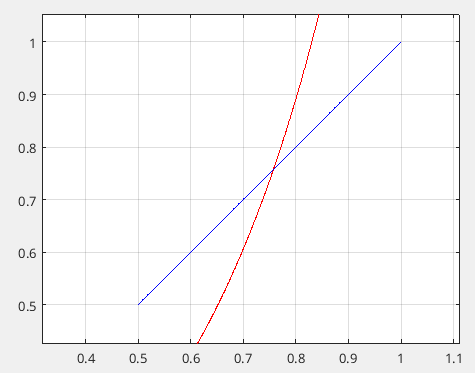
\includegraphics[width=0.6\textwidth]{images/code_fixed_bisector2.png}            
        \end{center}